%\nonstopmode
\hbadness=100000
\documentclass[a4paper, 12pt]{article}
\usepackage{amsmath,amsfonts,caption,float,geometry,graphicx,mathtools,pythonhighlight,textcomp,url,verbatim,subcaption,tabularx, longtable, ulem, hyperref, tikz, epigraph} %,parskip
\usetikzlibrary{automata, positioning}
\geometry{ a4paper, total={170mm,257mm}, left=20mm, top=20mm}
\newcommand{\matr}[1]{\underline{\underline{\textbf{#1}}}}
\newcommand{\ve}[1]{\boldsymbol{#1}}
\newcommand{\pythoncode}[2]{
\DeclareMathOperator*{\argmax}{arg\,max}
\DeclareMathOperator*{\argmin}{arg\,min}
\begin{adjustwidth}{-1.3cm}{-1.3cm}
\texttt{#1}
\inputpython{#2}{1}{1500}
\end{adjustwidth}
}
\usepackage[toc, page]{appendix}
% \usepackage[dvipsnames]{xcolor}
% \definecolor{subr}{rgb}{0.8, 0.33, 0.0}
% \definecolor{func}{rgb}{0.76, 0.6, 0.42}

\begin{document}
% \includegraphics[width=8cm]{CoverPage/UoBlogo.pdf}
% \hrule
% \bigbreak
% \textbf{F}usion Neutron \textbf{Acti}vation Spectra \textbf{U}nfolding by \textbf{N}eural \textbf{N}etworks \\
% (FACTIUNN)                                      \\
% \hrule
% \bigbreak
% \begin{minipage}[b]{0.4\textwidth}
%     \includegraphics[height=2cm]{CoverPage/CCFElogo.jpeg}
%   \end{minipage}
%   \hfill
%   \begin{minipage}[b]{0.4\textwidth}
%     \includegraphics[height=3cm]{CoverPage/UKAEAlogo.jpeg}
% \end{minipage}
    
\begin{table}[!h]
\centering
\begin{tabular}{rl}
author:&Ocean Wong          \\
       &(Hoi Yeung Wong)    \\
supervisor:&Chantal Nobs    \\
           &Robin Smith     \\
date:  &December 2019       \\
Organization:&Culham Centre for Fusion Energy\\
            &and Sheffield Hallam University
\end{tabular}
\end{table}
\hrule
\bigbreak
\abstract ENDF is a format for storing nuclear data. It is widely used in nuclear industries and academia, but it not-at-all human-readable, despite being written in plain text. This text is written as a quick start guide for the average physicist; it assumes the reader has some understanding of nuclear reactions, but has never seen an ENDF file.
%Very intimidating for the average nuclear physicist who would like to use it for the first time.
%This text aims to bridge the gap between the two, without providing any technical details into the usage of it.

\begin{center}
\chapter{A gentle introduction into ENDF}
\end{center}
\section{MT and MF numbers}
\begin{enumerate}
    \item For each nuclide in the Segr\'{e} chart, in its excited or ground state; \label{MAT number}
    \item Multiple reactions can occur upon impact with a variety of projectiles;\label{MT number}
    \item And each reaction must be characterized by its probability distribution with respect to
    \begin{itemize} \label{MF number}
         \item angle,
         \item energy,
         \item underlying mechanism,
         \item ... etc.
         \item and covariance matrix (uncertainty) of each
     \end{itemize} 
\end{enumerate}

To deal with point \ref{MAT number}, an identifying number $1\le$\texttt{MAT}$\le9999$ is assigned to each isomer.

To deal with point \ref{MT number}, an identifying number $1\le$\texttt{MT}$\le999$ is assigned to each reaction.
A different MT number is assigned for each unique combination of incoming projectile + out-going particle.
The full MT number table can be found in \href{https://www.oecd-nea.org/dbdata/data/manual-endf/endf102_MT.pdf}{Appendix B of the ENDF manual}.

Dealing with point \ref{MF number} is more subtle. Instead of storing its probability of reaction(or reaction cross-section) as a scalar function with n input dimensions, where $n>3$ (mechanism, angle, energy, decay time, etc.), which is going to be sparsely populated anyways, they are recorded as 1-dimensional lists of numbers (or, in the case of covariance matrices, 2-dimensional matrices of numbers), each list is given a number $1\le$\texttt{MF}$\le40$. For example, MF=3 records the reaction cross-section $\sigma(E)$ as a function of energy $E$ (integrated over all solid angle); MF=4 records the probability of emission $P(\theta)$ as a function of angle $\theta$ (fixed at $E= \frac{1}{40}eV$), etc. See Table \ref{MF table} below for more details.

\begin{table}[H]
\begin{tabular}{l|cccc}
MF\textbackslash MT         & 1(n,total)&2(z,z$_0$)&4(z,n) &151(n,RES) \\
\hline
1(General information)      &           &       &       &Resonance region (*)\\
2(Resonance param. data) & & & &effective scattering radius\\
3(Reaction cross-section)   &$\sigma_T(E)$      &$\sigma_{\text{elas}}(E)$     & $\sigma_{(n,2n)}(E)$& $\sigma(E_{RES})$ (a scalar)\\
4(Angular distributions)    &N/A& $P(\theta_{\text{scattered n.}})$& $P(\theta_{\text{expelled n.'s}})$ &N/A\\
5(Energy distributions)     &N/A& $P(E_{\text{scattered n.}})$     & $P(E_{\text{expelled n.'s}})$ &N/A
\end{tabular}
\caption{For each isomer, each MT number denotes a possible reaction, and each MF number denotes what information is required to characterize this reaction.} \label{MF-MT table}
\end{table}
See footnote\footnote{`Resonance parameters that can be used to calculate cross sections at different temperatures in the resolved and unresolved energy regions.'\cite{ENDFmanual}\href{https://www.oecd-nea.org/dbdata/data/manual-endf/endf102_MT.pdf}{Appendix B, which is directly linked here.}} for explanation on * in Table \ref{MF-MT table}.

A more tangible example is listed as follows: to get the angular distribution of non-elastically scattered neutrons from $^1$H, we should look for 
\begin{enumerate}
    \item MAT=1001,
    \item MT=3 (non-elastic neutron cross-section),
    \item MF=4 (Angular distributions for emitted particles).
\end{enumerate}

The complete MF table is included below for the reader's reference.

\begin{table}[H]
\centering
\begin{tabular}{ll}
MF&Description\\
\hline
1 &General information\\
2 &Resonance parameter data\\
3 &Reaction cross-sections\\
4 &Angular distributions for emitted particles\\
5 &Energy distributions for emitted particles\\
6 &Energy-angle distributions for emitted particles\\
7 &Thermal neutron scattering law data\\
8 &Radioactivity and fission-product yield data\\
9 &Multiplicities for radioactive nuclide production\\
10&Cross-sections for radioactive nuclide production\\
12&Multiplicities for photon production\\
13&Cross-sections for photon production\\
14&Angular distributions for photon production\\
15&Energy distributions for photon production\\
23&Photo- or electro-atomic interaction cross-sections\\
26&Electro-atomic angle and energy distribution\\
27&Atomic form factors or scattering functions for photo-atomic interactions\\
28&Atomic relaxation data\\
30&Data covariances obtained from parameter covariances and sensitivities\\
31&Data covariances for nu(bar)\\
32&Data covariances for resonance parameters\\
33&Data covariances for reaction cross-sections\\
34&Data covariances for angular distributions\\
35&Data covariances for energy distributions\\
39&Data covariances for radionuclide production yields\\
40&Data covariances for radionuclide production cross-sections
\end{tabular}
\caption{The complete MF number table as copied from the ENDF manual's ``Table 3"\cite{ENDFmanual}, for the reader's reference. Some values are unused as they are deprecated.}\label{MF table}
\end{table}

Therefore each ENDF ``File" must have an MAT number, an MT number, and an MF number associated with it.

\section{A simple illustration of the typical ENDF database layout}
Perhaps the most misleading word in the whole ENDF nomenclature is the word ``file": In the modern days of computing, it should really be called a ``section within a text file" to prevent confusion.

As stated in section 0.4.2 of \cite{ENDFmanual}: A ``File" refers to `a block of data in an evaluation that describes a certain data type'.

Here, each `data type' refers to an aspect of a nuclear reaction:\\e.g. for the case of inelastic neutron scattering, the angular distribution of the outgoing neutron is a `data type'.
\\(MT=51
(n,n')
, MF=6
(energy-angle distributions for emitted particles)
) 
% $^{56}_{26}$Fe

Concatenating multiple ENDF ``Files" together gives a computer-readable text file. From this point onwards, you can safely assume that, whenever the word file appears without quotation marks, I am using the universal definition of a regular text file, whose end-of-file byte position is indicated by a EOF character.

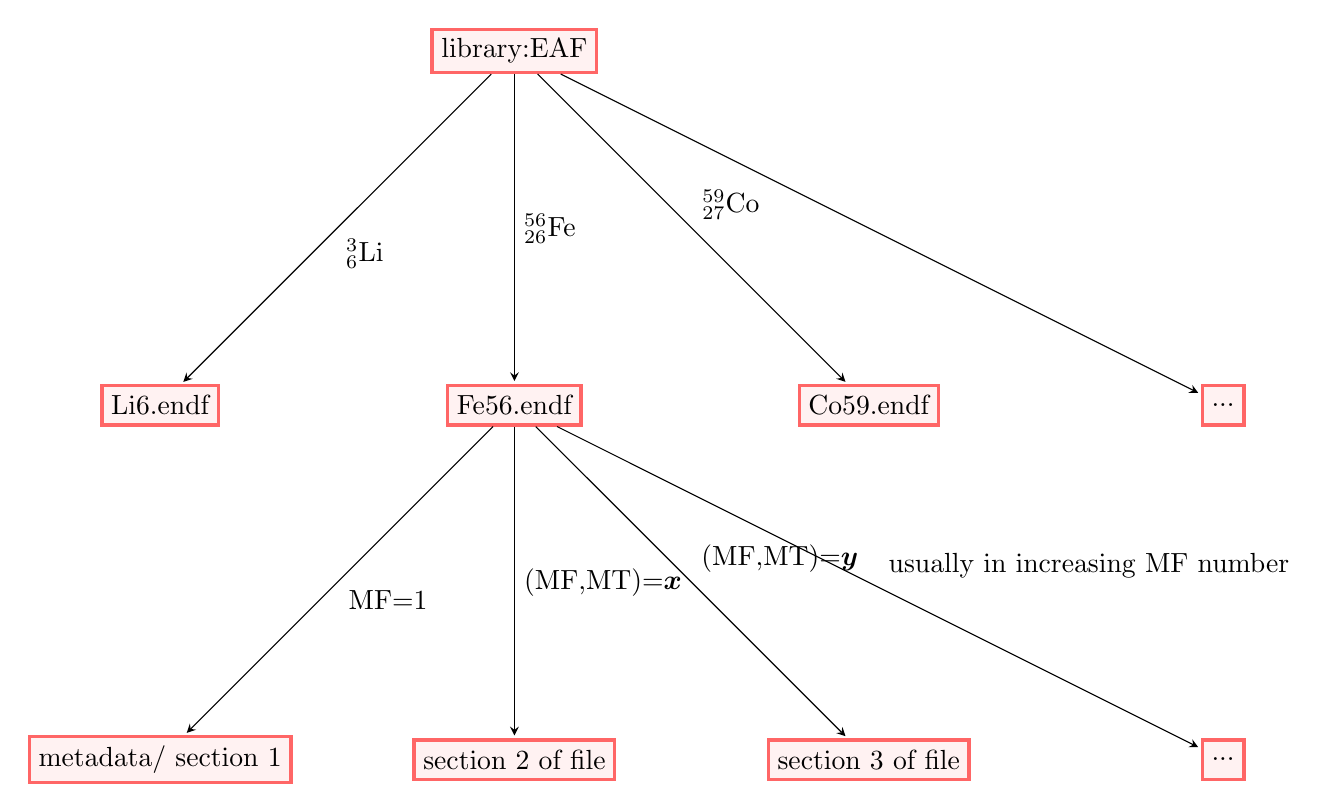
\begin{tikzpicture}%
  [>=stealth,
   shorten >=1pt,
   node distance=4.5cm,
   on grid,
   auto,
squarednode/.style={rectangle, draw=red!60, fill=red!5, very thick, minimum size=5mm},  ]
\node[squarednode] (root)            {library:EAF};
\node[squarednode] (lower) [below=of root] {Fe56.endf};
\node[squarednode] (left)  [left=of lower] {Li6.endf};
\node[squarednode] (right) [right=of lower] {Co59.endf};
\node[squarednode] (moreright) [right=of right] {...};
\node[squarednode] (midsec)[below=of lower] {section 2 of file};
\node[squarednode] (topsec)[left=of midsec] {metadata/ section 1};
\node[squarednode] (botsec)[right=of midsec] {section 3 of file};
\node[squarednode] (rigsec)[right=of botsec] {...};

\path[->]
%   FROM       BEND/LOOP           POSITION OF LABEL   LABEL   TO
   (root)  edge                node                      {$^{3 }_{6 }$Li} (left)
           edge                node                      {$^{56}_{26}$Fe} (lower)
           edge                node                      {$^{59}_{27}$Co} (right)
           edge                node                      {} (moreright)
   (lower) edge                node                      {MF=1} (topsec)
   (lower) edge                node                      {(MF,MT)=$\ve{x}$} (midsec)
   (lower) edge                node                      {(MF,MT)=$\ve{y}$} (botsec)
   (lower) edge                node                      {usually in increasing MF number} (rigsec)
   ;
\end{tikzpicture}
The layout of the EAF library is illustrated above. The root (library:EAF) is the folder containing everything.

Inside the folder are files, named after each isotope. Each file contains some data about that element; but it rarely contains data of \emph{all} 999 MT numbers $\times$ 40 MF numbers.

Inside each file are sections, each corresponding to a set of MT and MF numbers.

This is not the only way to organize the files and folders.
\begin{itemize}
    \item ENDF files don't always have to end in ``.endf"; as long as it is written in the same format as specified by \cite{ENDFmanual} in ASCII text, it can be read by \texttt{OpenMC}/\texttt{pyne}.
    \item each file shown above actually consist of a collection of the ENDF ``Files" referenced by section 0.4.2 of \cite{ENDFmanual}, concatenated together.
    \item One can even concatenate all of the files in the 2nd layer into a single, very long (hundreds of MB's) text file with an arbitrary file extension.
    \item Some of the more comprehensive libraries (e.g. JEFF) records data across a large range of MT numbers; therefore they may split their libraries into multiple roots. For example, the \href{https://www-nds.iaea.org/public/download-endf/TENDL-2017/}{2017 release of TENDL} splits it into seven roots, sorted by projectile types:
    \begin{itemize}
        \item \texttt{library:TENDL/d}
        \item \texttt{library:TENDL/n}
        \item \texttt{library:TENDL/g} (gamma)
        \item \texttt{library:TENDL/he3}
        \item \texttt{library:TENDL/he4}
        \item \texttt{library:TENDL/p}
        \item \texttt{library:TENDL/t}
    \end{itemize}
    instead of a single root as shown in the EAF example above.
    \item You may also see the words ``ACE" file frequently occurring in the context of ENDF data. This stands for \underline{A} \underline{C}ompact \underline{E}NDF, which is the format that is fed into MCNP simulations. (Normal ENDF files are too big to be used in MCNP.)
\end{itemize}

\section{Using ENDF files}
The purpose of this text is not to provide the technical know-how of designing and writing ENDF files; but to simply give the average nuclear data user, who has no intention of becoming a nuclear cross-section evaluator, an idea of how to use the publicly available ENDF files. Therefore this section will introduce the easiest approach(es) to extracting data from ENDF files.

\subsection{The python approach}
Simply download an archive of ENDF files from \href{https://www-nds.iaea.org/public/download-endf}{any official website} of your choice, unzip it  into your working directory, and read it into memory using a nuclear data management package of your choice (\texttt{openmc} or \texttt{pyne}). These will then be saved as instances of a class(e.g. an \verb|openmc.data.endf.Evaluation|
object), where values such as $\sigma(E)$ will be saved as its attributes.

\bibliographystyle{plain}
\bibliography{ENDF}
\end{document}

\begin{appendices}
\end{appendices}
%`